\documentclass[]{article}
\usepackage{lmodern}
\usepackage{amssymb,amsmath}
\usepackage{ifxetex,ifluatex}
\usepackage{fixltx2e} % provides \textsubscript
\ifnum 0\ifxetex 1\fi\ifluatex 1\fi=0 % if pdftex
  \usepackage[T1]{fontenc}
  \usepackage[utf8]{inputenc}
\else % if luatex or xelatex
  \ifxetex
    \usepackage{mathspec}
  \else
    \usepackage{fontspec}
  \fi
  \defaultfontfeatures{Ligatures=TeX,Scale=MatchLowercase}
\fi
% use upquote if available, for straight quotes in verbatim environments
\IfFileExists{upquote.sty}{\usepackage{upquote}}{}
% use microtype if available
\IfFileExists{microtype.sty}{%
\usepackage{microtype}
\UseMicrotypeSet[protrusion]{basicmath} % disable protrusion for tt fonts
}{}
\usepackage[margin=1in]{geometry}
\usepackage{hyperref}
\hypersetup{unicode=true,
            pdftitle={Preliminary EDA},
            pdfborder={0 0 0},
            breaklinks=true}
\urlstyle{same}  % don't use monospace font for urls
\usepackage{color}
\usepackage{fancyvrb}
\newcommand{\VerbBar}{|}
\newcommand{\VERB}{\Verb[commandchars=\\\{\}]}
\DefineVerbatimEnvironment{Highlighting}{Verbatim}{commandchars=\\\{\}}
% Add ',fontsize=\small' for more characters per line
\usepackage{framed}
\definecolor{shadecolor}{RGB}{248,248,248}
\newenvironment{Shaded}{\begin{snugshade}}{\end{snugshade}}
\newcommand{\KeywordTok}[1]{\textcolor[rgb]{0.13,0.29,0.53}{\textbf{#1}}}
\newcommand{\DataTypeTok}[1]{\textcolor[rgb]{0.13,0.29,0.53}{#1}}
\newcommand{\DecValTok}[1]{\textcolor[rgb]{0.00,0.00,0.81}{#1}}
\newcommand{\BaseNTok}[1]{\textcolor[rgb]{0.00,0.00,0.81}{#1}}
\newcommand{\FloatTok}[1]{\textcolor[rgb]{0.00,0.00,0.81}{#1}}
\newcommand{\ConstantTok}[1]{\textcolor[rgb]{0.00,0.00,0.00}{#1}}
\newcommand{\CharTok}[1]{\textcolor[rgb]{0.31,0.60,0.02}{#1}}
\newcommand{\SpecialCharTok}[1]{\textcolor[rgb]{0.00,0.00,0.00}{#1}}
\newcommand{\StringTok}[1]{\textcolor[rgb]{0.31,0.60,0.02}{#1}}
\newcommand{\VerbatimStringTok}[1]{\textcolor[rgb]{0.31,0.60,0.02}{#1}}
\newcommand{\SpecialStringTok}[1]{\textcolor[rgb]{0.31,0.60,0.02}{#1}}
\newcommand{\ImportTok}[1]{#1}
\newcommand{\CommentTok}[1]{\textcolor[rgb]{0.56,0.35,0.01}{\textit{#1}}}
\newcommand{\DocumentationTok}[1]{\textcolor[rgb]{0.56,0.35,0.01}{\textbf{\textit{#1}}}}
\newcommand{\AnnotationTok}[1]{\textcolor[rgb]{0.56,0.35,0.01}{\textbf{\textit{#1}}}}
\newcommand{\CommentVarTok}[1]{\textcolor[rgb]{0.56,0.35,0.01}{\textbf{\textit{#1}}}}
\newcommand{\OtherTok}[1]{\textcolor[rgb]{0.56,0.35,0.01}{#1}}
\newcommand{\FunctionTok}[1]{\textcolor[rgb]{0.00,0.00,0.00}{#1}}
\newcommand{\VariableTok}[1]{\textcolor[rgb]{0.00,0.00,0.00}{#1}}
\newcommand{\ControlFlowTok}[1]{\textcolor[rgb]{0.13,0.29,0.53}{\textbf{#1}}}
\newcommand{\OperatorTok}[1]{\textcolor[rgb]{0.81,0.36,0.00}{\textbf{#1}}}
\newcommand{\BuiltInTok}[1]{#1}
\newcommand{\ExtensionTok}[1]{#1}
\newcommand{\PreprocessorTok}[1]{\textcolor[rgb]{0.56,0.35,0.01}{\textit{#1}}}
\newcommand{\AttributeTok}[1]{\textcolor[rgb]{0.77,0.63,0.00}{#1}}
\newcommand{\RegionMarkerTok}[1]{#1}
\newcommand{\InformationTok}[1]{\textcolor[rgb]{0.56,0.35,0.01}{\textbf{\textit{#1}}}}
\newcommand{\WarningTok}[1]{\textcolor[rgb]{0.56,0.35,0.01}{\textbf{\textit{#1}}}}
\newcommand{\AlertTok}[1]{\textcolor[rgb]{0.94,0.16,0.16}{#1}}
\newcommand{\ErrorTok}[1]{\textcolor[rgb]{0.64,0.00,0.00}{\textbf{#1}}}
\newcommand{\NormalTok}[1]{#1}
\usepackage{graphicx,grffile}
\makeatletter
\def\maxwidth{\ifdim\Gin@nat@width>\linewidth\linewidth\else\Gin@nat@width\fi}
\def\maxheight{\ifdim\Gin@nat@height>\textheight\textheight\else\Gin@nat@height\fi}
\makeatother
% Scale images if necessary, so that they will not overflow the page
% margins by default, and it is still possible to overwrite the defaults
% using explicit options in \includegraphics[width, height, ...]{}
\setkeys{Gin}{width=\maxwidth,height=\maxheight,keepaspectratio}
\IfFileExists{parskip.sty}{%
\usepackage{parskip}
}{% else
\setlength{\parindent}{0pt}
\setlength{\parskip}{6pt plus 2pt minus 1pt}
}
\setlength{\emergencystretch}{3em}  % prevent overfull lines
\providecommand{\tightlist}{%
  \setlength{\itemsep}{0pt}\setlength{\parskip}{0pt}}
\setcounter{secnumdepth}{0}
% Redefines (sub)paragraphs to behave more like sections
\ifx\paragraph\undefined\else
\let\oldparagraph\paragraph
\renewcommand{\paragraph}[1]{\oldparagraph{#1}\mbox{}}
\fi
\ifx\subparagraph\undefined\else
\let\oldsubparagraph\subparagraph
\renewcommand{\subparagraph}[1]{\oldsubparagraph{#1}\mbox{}}
\fi

%%% Use protect on footnotes to avoid problems with footnotes in titles
\let\rmarkdownfootnote\footnote%
\def\footnote{\protect\rmarkdownfootnote}

%%% Change title format to be more compact
\usepackage{titling}

% Create subtitle command for use in maketitle
\newcommand{\subtitle}[1]{
  \posttitle{
    \begin{center}\large#1\end{center}
    }
}

\setlength{\droptitle}{-2em}

  \title{Preliminary EDA}
    \pretitle{\vspace{\droptitle}\centering\huge}
  \posttitle{\par}
    \author{}
    \preauthor{}\postauthor{}
    \date{}
    \predate{}\postdate{}
  

\begin{document}
\maketitle

\begin{Shaded}
\begin{Highlighting}[]
\KeywordTok{library}\NormalTok{(}\StringTok{'tidyverse'}\NormalTok{)}
\end{Highlighting}
\end{Shaded}

\begin{verbatim}
## -- Attaching packages -------------------------------------------------------------------------- tidyverse 1.2.1 --
\end{verbatim}

\begin{verbatim}
## √ ggplot2 3.0.0     √ purrr   0.2.5
## √ tibble  1.4.2     √ dplyr   0.7.6
## √ tidyr   0.8.1     √ stringr 1.3.1
## √ readr   1.1.1     √ forcats 0.3.0
\end{verbatim}

\begin{verbatim}
## -- Conflicts ----------------------------------------------------------------------------- tidyverse_conflicts() --
## x dplyr::filter() masks stats::filter()
## x dplyr::lag()    masks stats::lag()
\end{verbatim}

\begin{Shaded}
\begin{Highlighting}[]
\NormalTok{frmgham <-}\StringTok{ }\KeywordTok{read_csv}\NormalTok{(}\StringTok{'frmgham2.csv'}\NormalTok{)}
\end{Highlighting}
\end{Shaded}

\begin{verbatim}
## Parsed with column specification:
## cols(
##   .default = col_integer(),
##   SYSBP = col_double(),
##   DIABP = col_double(),
##   BMI = col_double()
## )
\end{verbatim}

\begin{verbatim}
## See spec(...) for full column specifications.
\end{verbatim}

\begin{Shaded}
\begin{Highlighting}[]
\NormalTok{frmgham_kaggle <-}\StringTok{ }\KeywordTok{read_csv}\NormalTok{(}\StringTok{'framingham.csv'}\NormalTok{)}
\end{Highlighting}
\end{Shaded}

\begin{verbatim}
## Parsed with column specification:
## cols(
##   male = col_integer(),
##   age = col_integer(),
##   education = col_integer(),
##   currentSmoker = col_integer(),
##   cigsPerDay = col_integer(),
##   BPMeds = col_integer(),
##   prevalentStroke = col_integer(),
##   prevalentHyp = col_integer(),
##   diabetes = col_integer(),
##   totChol = col_integer(),
##   sysBP = col_double(),
##   diaBP = col_double(),
##   BMI = col_double(),
##   heartRate = col_integer(),
##   glucose = col_integer(),
##   TenYearCHD = col_integer()
## )
\end{verbatim}

\begin{Shaded}
\begin{Highlighting}[]
\KeywordTok{problems}\NormalTok{(frmgham)}
\end{Highlighting}
\end{Shaded}

\begin{verbatim}
## # tibble [0 x 4]
## # ... with 4 variables: row <int>, col <int>, expected <chr>, actual <chr>
\end{verbatim}

\begin{Shaded}
\begin{Highlighting}[]
\KeywordTok{problems}\NormalTok{(frmgham_kaggle)}
\end{Highlighting}
\end{Shaded}

\begin{verbatim}
## # tibble [0 x 4]
## # ... with 4 variables: row <int>, col <int>, expected <chr>, actual <chr>
\end{verbatim}

\subsection{Intial Analysis}\label{intial-analysis}

\begin{Shaded}
\begin{Highlighting}[]
\NormalTok{pop_tb <-}\StringTok{ }\KeywordTok{as.data.frame}\NormalTok{(}\KeywordTok{table}\NormalTok{(frmgham}\OperatorTok{$}\NormalTok{AGE, frmgham}\OperatorTok{$}\NormalTok{SEX))}
\NormalTok{pop_tb}
\end{Highlighting}
\end{Shaded}

\begin{verbatim}
##     Var1 Var2 Freq
## 1     32    1    0
## 2     33    1    2
## 3     34    1    5
## 4     35    1   17
## 5     36    1   43
## 6     37    1   45
## 7     38    1   70
## 8     39    1   76
## 9     40    1   88
## 10    41    1   94
## 11    42    1  116
## 12    43    1  120
## 13    44    1  153
## 14    45    1  147
## 15    46    1  154
## 16    47    1  144
## 17    48    1  199
## 18    49    1  157
## 19    50    1  209
## 20    51    1  193
## 21    52    1  197
## 22    53    1  178
## 23    54    1  214
## 24    55    1  156
## 25    56    1  180
## 26    57    1  179
## 27    58    1  171
## 28    59    1  138
## 29    60    1  173
## 30    61    1  137
## 31    62    1  151
## 32    63    1  150
## 33    64    1  133
## 34    65    1  122
## 35    66    1   97
## 36    67    1  109
## 37    68    1   94
## 38    69    1   83
## 39    70    1   65
## 40    71    1   52
## 41    72    1   50
## 42    73    1   45
## 43    74    1   42
## 44    75    1   25
## 45    76    1   24
## 46    77    1   12
## 47    78    1    4
## 48    79    1    6
## 49    80    1    3
## 50    81    1    0
## 51    32    2    1
## 52    33    2    3
## 53    34    2   13
## 54    35    2   25
## 55    36    2   41
## 56    37    2   48
## 57    38    2   75
## 58    39    2  102
## 59    40    2  124
## 60    41    2  119
## 61    42    2  142
## 62    43    2  136
## 63    44    2  151
## 64    45    2  192
## 65    46    2  226
## 66    47    2  198
## 67    48    2  227
## 68    49    2  210
## 69    50    2  217
## 70    51    2  255
## 71    52    2  273
## 72    53    2  255
## 73    54    2  250
## 74    55    2  243
## 75    56    2  216
## 76    57    2  207
## 77    58    2  233
## 78    59    2  229
## 79    60    2  209
## 80    61    2  211
## 81    62    2  190
## 82    63    2  207
## 83    64    2  188
## 84    65    2  168
## 85    66    2  140
## 86    67    2  157
## 87    68    2  122
## 88    69    2  109
## 89    70    2  104
## 90    71    2   90
## 91    72    2   60
## 92    73    2   62
## 93    74    2   48
## 94    75    2   46
## 95    76    2   27
## 96    77    2   21
## 97    78    2   14
## 98    79    2   15
## 99    80    2    3
## 100   81    2    3
\end{verbatim}

\begin{Shaded}
\begin{Highlighting}[]
\KeywordTok{names}\NormalTok{(pop_tb)[}\DecValTok{1}\NormalTok{] <-}\StringTok{ }\KeywordTok{paste}\NormalTok{(}\StringTok{"Age"}\NormalTok{)}
\KeywordTok{names}\NormalTok{(pop_tb)[}\DecValTok{2}\NormalTok{] <-}\StringTok{ }\KeywordTok{paste}\NormalTok{(}\StringTok{"Gender"}\NormalTok{)}

\NormalTok{pop_tb}\OperatorTok{$}\NormalTok{Age <-}\StringTok{ }\KeywordTok{as.numeric}\NormalTok{(}\KeywordTok{as.character}\NormalTok{(pop_tb}\OperatorTok{$}\NormalTok{Age))}


\CommentTok{# Plot Age Range with respective Frequencies and label with Gender orientation}
\KeywordTok{ggplot}\NormalTok{(pop_tb, }\KeywordTok{aes}\NormalTok{(}\DataTypeTok{x =}\NormalTok{ Age, }\DataTypeTok{y =}\NormalTok{ Freq, }\DataTypeTok{fill =}\NormalTok{ Gender)) }\OperatorTok{+}
\StringTok{ }\CommentTok{# Define each gender in barplot distribution}
\KeywordTok{geom_bar}\NormalTok{(}\DataTypeTok{data =} \KeywordTok{subset}\NormalTok{(pop_tb, Gender }\OperatorTok{==}\StringTok{ }\DecValTok{1}\NormalTok{), }\DataTypeTok{stat =} \StringTok{"identity"}\NormalTok{, }\DataTypeTok{mapping =} \KeywordTok{aes}\NormalTok{(}\DataTypeTok{y =}\NormalTok{ Freq), }\DataTypeTok{color=}\StringTok{"grey"}\NormalTok{, }\DataTypeTok{size=}\FloatTok{0.2}\NormalTok{) }\OperatorTok{+}
\StringTok{ }\KeywordTok{geom_bar}\NormalTok{(}\DataTypeTok{data =} \KeywordTok{subset}\NormalTok{(pop_tb, Gender }\OperatorTok{==}\StringTok{ }\DecValTok{2}\NormalTok{), }\DataTypeTok{stat =} \StringTok{"identity"}\NormalTok{, }\DataTypeTok{position =} \StringTok{"identity"}\NormalTok{, }\DataTypeTok{mapping =} \KeywordTok{aes}\NormalTok{(}\DataTypeTok{y =} \OperatorTok{-}\NormalTok{Freq), }\DataTypeTok{color=}\StringTok{"grey"}\NormalTok{, }\DataTypeTok{size=}\FloatTok{0.2}\NormalTok{) }\OperatorTok{+}
\StringTok{ }\CommentTok{# Define the limits on scales}

\StringTok{ }\CommentTok{# Turn to horizontal barplots}
\StringTok{ }\KeywordTok{coord_flip}\NormalTok{() }\OperatorTok{+}
\StringTok{ }\CommentTok{# Title, Legend}
\StringTok{ }\KeywordTok{theme_bw}\NormalTok{() }\OperatorTok{+}
\StringTok{ }\KeywordTok{xlab}\NormalTok{(}\StringTok{"Age (years)"}\NormalTok{) }\OperatorTok{+}
\StringTok{ }\KeywordTok{ylab}\NormalTok{(}\StringTok{"Total of Patients"}\NormalTok{) }\OperatorTok{+}
\StringTok{ }\KeywordTok{ggtitle}\NormalTok{(}\StringTok{"Distribution of Patients by Age and Gender"}\NormalTok{)}
\end{Highlighting}
\end{Shaded}

\includegraphics{Pre_EDA_files/figure-latex/ind-1.pdf} From the graph,
we can see that there are more females(green) then males(orange)
involved in this study. Participants were mainly distributed among age
45 -- 60. From the graph, we can know that females who are 52 years ago
and males who are 54 years ago are more likely to have heart disease.

Checking the distribution of different traits based on the education

\begin{Shaded}
\begin{Highlighting}[]
\NormalTok{frmgham }\OperatorTok\StringTok{ }\KeywordTok{group_by}\NormalTok{(educ) }\OperatorTok\StringTok{ }\KeywordTok{filter}\NormalTok{(}\OperatorTok{!}\KeywordTok{is.na}\NormalTok{(BMI),}\OperatorTok{!}\KeywordTok{is.na}\NormalTok{(educ)) }\OperatorTok\StringTok{ }\KeywordTok{summarise}\NormalTok{(}\DataTypeTok{mean_bmi=}\KeywordTok{mean}\NormalTok{(BMI))}
\end{Highlighting}
\end{Shaded}

\begin{verbatim}
## # A tibble: 4 x 2
##    educ mean_bmi
##   <int>    <dbl>
## 1     1     26.6
## 2     2     25.5
## 3     3     25.0
## 4     4     25.3
\end{verbatim}

\begin{Shaded}
\begin{Highlighting}[]
\NormalTok{frmgham }\OperatorTok\StringTok{ }\KeywordTok{group_by}\NormalTok{(educ) }\OperatorTok\StringTok{ }\KeywordTok{filter}\NormalTok{(}\OperatorTok{!}\KeywordTok{is.na}\NormalTok{(HEARTRTE),}\OperatorTok{!}\KeywordTok{is.na}\NormalTok{(educ)) }\OperatorTok\StringTok{ }\KeywordTok{summarise}\NormalTok{(}\DataTypeTok{mean_heart_rate=}\KeywordTok{mean}\NormalTok{(HEARTRTE))}
\end{Highlighting}
\end{Shaded}

\begin{verbatim}
## # A tibble: 4 x 2
##    educ mean_heart_rate
##   <int>           <dbl>
## 1     1            77.0
## 2     2            77.6
## 3     3            76.8
## 4     4            74.2
\end{verbatim}

\begin{Shaded}
\begin{Highlighting}[]
\NormalTok{frmgham }\OperatorTok\StringTok{ }\KeywordTok{group_by}\NormalTok{(educ) }\OperatorTok\StringTok{ }\KeywordTok{filter}\NormalTok{(}\OperatorTok{!}\KeywordTok{is.na}\NormalTok{(GLUCOSE),}\OperatorTok{!}\KeywordTok{is.na}\NormalTok{(educ)) }\OperatorTok\StringTok{ }\KeywordTok{summarise}\NormalTok{(}\DataTypeTok{mean_glucose=}\KeywordTok{mean}\NormalTok{(GLUCOSE))}
\end{Highlighting}
\end{Shaded}

\begin{verbatim}
## # A tibble: 4 x 2
##    educ mean_glucose
##   <int>        <dbl>
## 1     1         85.9
## 2     2         83.3
## 3     3         83.0
## 4     4         82.3
\end{verbatim}

\subsection{Discussion for initial
analysis}\label{discussion-for-initial-analysis}

we analysed the framigham data set to check how a socieconomic status
and access to higher levels of education affected factors such as
bmi(body mass index),heart rate and glucose level(we assessed glucose
levels because constant high glucose level(hyperglycemia) are correlated
with high risk for certain lifestyle diseases.

BMI: From our assesment, higher levels of education are associated a
lower mean bmi. The bmi increased as education levels decreased: An
education level of 1 is associated with the highest bmi which would be
expected to put this group at the highest risk for lifestyle diseases
such as CHD, stroke, high bloop pressure and diabetes.

Overall, a lower heart rate at rest indicated more efficient heart
function and better cardiovascular fitness and vice-versa. Heart Rate:
As would be expected, the lowest levels of education would be associated
with the highest heart rate which in the long-run would put them at a
higher risk for diseases. The mean heart rate for each level of
education decreased as education levels increased.

Blood glucose levels range from 90 to 130 mg/dL before meals, and below
180 mg/dL within 1 to 2 hours after a meal. In general, most people
without diabetes have blood sugar levels before meals hover around 70 to
80 mg/dL: 60 is normal; for others, 90.Hypoglycemia, also called low
blood glucose or low blood sugar, occurs when the level of glucose in
your blood drops below normal. For many people with diabetes, that means
a level of 70 milligrams per deciliter (mg/dL) or less. Glucose: the
mean glucose levels decreased as education levels increased. Higher
education levels were assocaited with lower and slightly healthier
glucose levels. Overall, the mean glucose levels for all groups were
fell within a healthy range for glucose levels.

\subsection{Logistic Models}\label{logistic-models}

Some of the early logistic models

\begin{Shaded}
\begin{Highlighting}[]
\CommentTok{#Predicting presence of Coronary Heart Disease using risk factors}
\NormalTok{beta <-}\StringTok{ }\KeywordTok{coef}\NormalTok{(}\KeywordTok{glm}\NormalTok{(PREVCHD }\OperatorTok{~}\StringTok{ }\NormalTok{BMI }\OperatorTok{+}\StringTok{ }\NormalTok{TOTCHOL }\OperatorTok{+}\StringTok{ }\NormalTok{AGE }\OperatorTok{+}\StringTok{ }\NormalTok{SYSBP }\OperatorTok{+}\StringTok{ }\NormalTok{GLUCOSE }\OperatorTok{+}\StringTok{ }\NormalTok{CIGPDAY }\OperatorTok{+}\StringTok{ }\NormalTok{LDLC,}\DataTypeTok{data=}\NormalTok{frmgham,}\DataTypeTok{family=}\KeywordTok{binomial}\NormalTok{()))}

\CommentTok{#Predicting prevalence of Stroke using risk factors}
\NormalTok{beta_}\DecValTok{1}\NormalTok{ <-}\StringTok{ }\KeywordTok{coef}\NormalTok{(}\KeywordTok{glm}\NormalTok{(PREVSTRK }\OperatorTok{~}\StringTok{ }\NormalTok{BMI }\OperatorTok{+}\StringTok{ }\NormalTok{TOTCHOL }\OperatorTok{+}\StringTok{ }\NormalTok{AGE }\OperatorTok{+}\StringTok{ }\NormalTok{SYSBP }\OperatorTok{+}\StringTok{ }\NormalTok{DIABP }\OperatorTok{+}\StringTok{ }\NormalTok{GLUCOSE }\OperatorTok{+}\StringTok{ }\NormalTok{CIGPDAY }\OperatorTok{+}\StringTok{ }\NormalTok{LDLC,}\DataTypeTok{data=}\NormalTok{frmgham,}\DataTypeTok{family=}\KeywordTok{binomial}\NormalTok{()))}

\NormalTok{preval_chd <-}\StringTok{ }\KeywordTok{as.tibble}\NormalTok{(}\KeywordTok{as.list}\NormalTok{(beta[}\OperatorTok{-}\DecValTok{1}\NormalTok{])) }\OperatorTok\StringTok{ }\KeywordTok{gather}\NormalTok{(risk_factor,coef)}

\NormalTok{preval_strk <-}\StringTok{ }\KeywordTok{as.tibble}\NormalTok{(}\KeywordTok{as.list}\NormalTok{(beta_}\DecValTok{1}\NormalTok{[}\OperatorTok{-}\DecValTok{1}\NormalTok{])) }\OperatorTok\StringTok{ }\KeywordTok{gather}\NormalTok{(risk_factor,coef)}

\KeywordTok{ggplot}\NormalTok{(preval_strk,}\KeywordTok{aes}\NormalTok{(}\KeywordTok{reorder}\NormalTok{(}\KeywordTok{factor}\NormalTok{(risk_factor), coef), coef)) }\OperatorTok{+}\StringTok{ }\KeywordTok{geom_point}\NormalTok{()}
\end{Highlighting}
\end{Shaded}

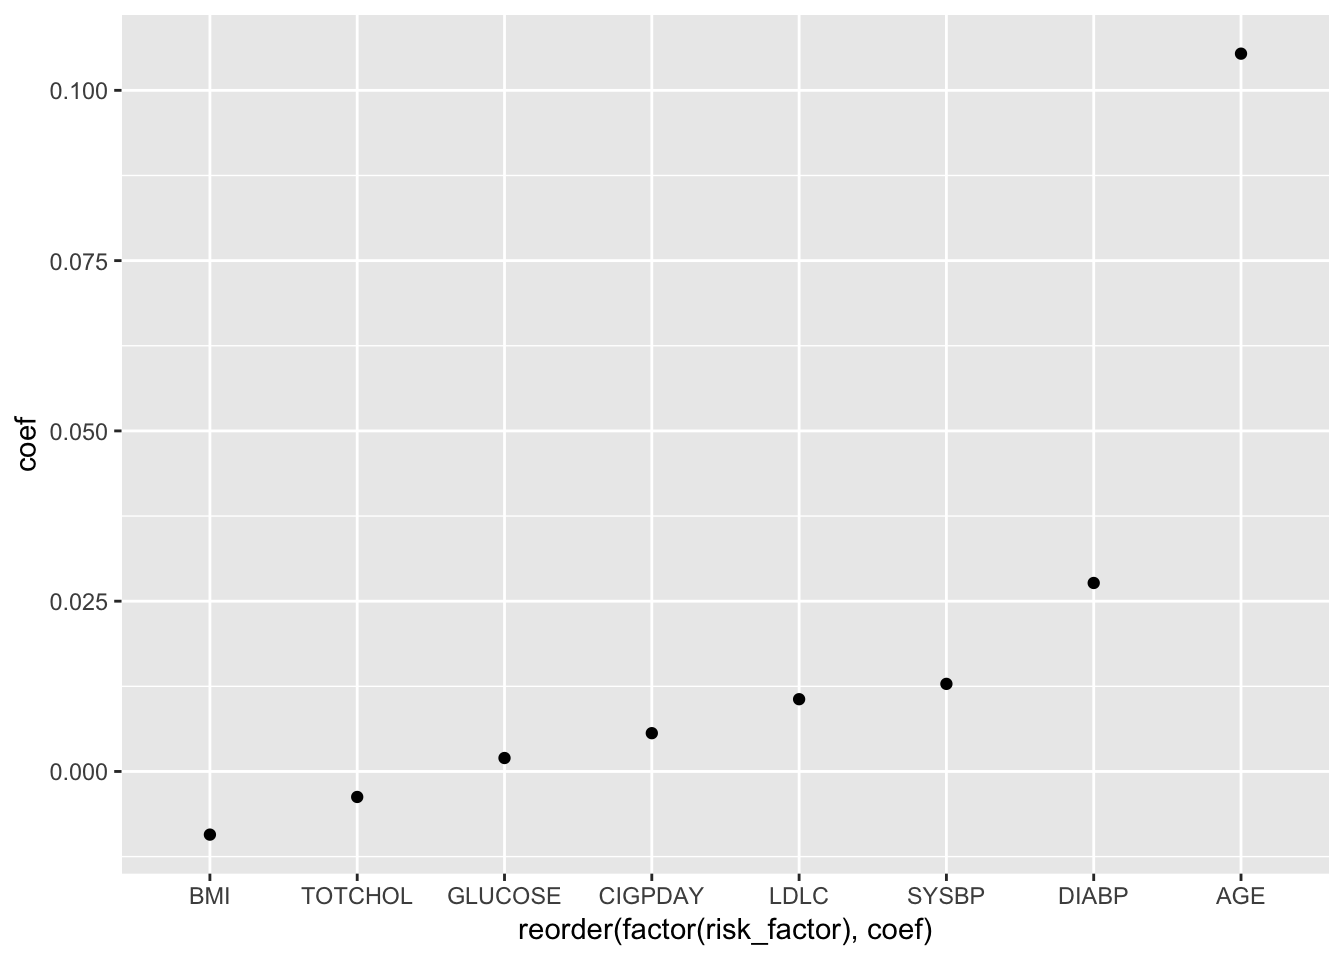
\includegraphics{Pre_EDA_files/figure-latex/logistic-1.pdf}

\begin{Shaded}
\begin{Highlighting}[]
\KeywordTok{ggplot}\NormalTok{(preval_chd,}\KeywordTok{aes}\NormalTok{(}\KeywordTok{reorder}\NormalTok{(}\KeywordTok{factor}\NormalTok{(risk_factor), coef), coef)) }\OperatorTok{+}\StringTok{ }\KeywordTok{geom_point}\NormalTok{()}
\end{Highlighting}
\end{Shaded}

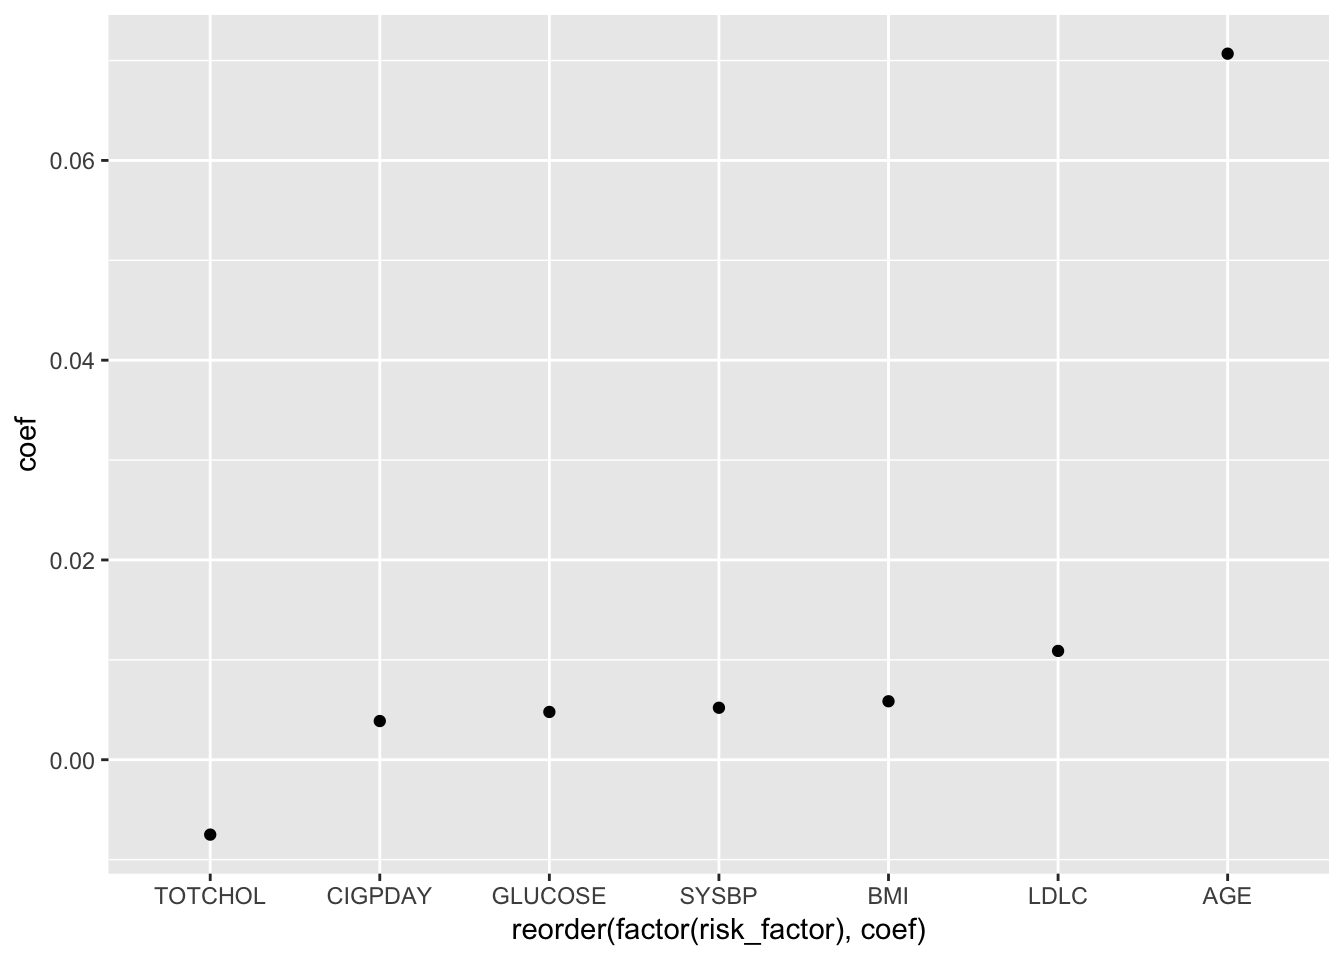
\includegraphics{Pre_EDA_files/figure-latex/logistic-2.pdf} \#\#
Discussion For this part,we used a logistic regression model to predict
the presence of Coronary Heart Disease using risk factors such as
BMIBody Mass Index(BMI), TOTCHOL(Total Cholestrol levels), AGE(Age),
Systolic Blood Pressure(SYSBP), GLUCOSE, the number of cigarettes per
day(CIGPDAY) and Blood levels of Low-density lipoprotein (LDL) is one of
the body's lipoproteins and an important carrier of cholesterol.LDL
cholesterol (LDL-C) are often assessed when evaluating the risk of
future heart disease.

AGE:From our model, age was the highest risk factor for predicting the
presence of Coronary Heart Disease. It would be expected that the older
one gets, the higher the risk for developing chronic and lifestyle
diseases.

Blood Pressure(BP):Blood Pressure is read in two readings. The first
reading(The top number)refers to the amount of pressure in your arteries
during the contraction of your heart muscle and is called systolic
pressure(SP:SYSBP). The second reading(the bottom number) refers to your
blood pressure when your heart muscle is between beats. This is called
diastolic pressure(DP: DIABP). A blood pressure less than 120/80 mmHg is
normal. A blood pressure of 140/90 mmHg or more is too high. People with
levels in between 120/80 and 140/90 have a condition called
prehypertension, which means they are at high risk for high blood
pressure. From our model, we assessed that the diastolic blood pressure
put one at a higher risk for presence of Coronary Heart Disease(after
AGE) more than the systolic blood pressure.

Another important distinction was noted between TOTAL CHOL level and
LDLC levels. One would expect higher levels of total cholestrol(TOTCHOL)
to be a higher predictor but using logistic regression model to asses
the framigham dataset, Higher Levels of Low-density lipoprotein (LDL)
put one at a higher risk of cornary heart disease more than the former.

Overall,Body Mass Index(BMI) was the lowest predictor for the presence
of Coronary Heart Disease.

Note that the \texttt{echo\ =\ FALSE} parameter was added to the code
chunk to prevent printing of the R code that generated the plot. \#\#
BMI Based Categorisation

\begin{Shaded}
\begin{Highlighting}[]
\NormalTok{frmgham_mod<-}\StringTok{ }\NormalTok{frmgham }\OperatorTok\StringTok{ }
\StringTok{  }\KeywordTok{mutate}\NormalTok{(}\DataTypeTok{BMI_Class=}\KeywordTok{case_when}\NormalTok{(BMI}\OperatorTok{<}\FloatTok{18.5}\OperatorTok{~}\StringTok{'Underweight'}\NormalTok{,BMI }\OperatorTok{>=}\StringTok{ }\FloatTok{18.5} \OperatorTok{&}\StringTok{ }\NormalTok{BMI }\OperatorTok{<}\DecValTok{25} \OperatorTok{~}\StringTok{ 'Normal'}\NormalTok{,BMI }\OperatorTok{>=}\StringTok{ }\DecValTok{25} \OperatorTok{&}\StringTok{ }\NormalTok{BMI }\OperatorTok{<}\StringTok{ }\DecValTok{30} \OperatorTok{~}\StringTok{ 'Overweight'}\NormalTok{,BMI}\OperatorTok{>=}\DecValTok{30} \OperatorTok{&}\StringTok{ }\NormalTok{BMI}\OperatorTok{<}\DecValTok{35} \OperatorTok{~}\StringTok{ 'Obese'}\NormalTok{,BMI}\OperatorTok{>=}\DecValTok{35} \OperatorTok{~}\StringTok{ 'Super Obese'}\NormalTok{)) }

\CommentTok{# SUMMARY OF Mean Heart Rates by BMI category}
\NormalTok{frmgham_mod }\OperatorTok\StringTok{ }\KeywordTok{group_by}\NormalTok{(BMI_Class) }\OperatorTok\StringTok{ }\KeywordTok{filter}\NormalTok{(}\OperatorTok{!}\KeywordTok{is.na}\NormalTok{(HEARTRTE) }\OperatorTok{&}\StringTok{ }\OperatorTok{!}\KeywordTok{is.na}\NormalTok{(BMI)) }\OperatorTok\StringTok{ }\KeywordTok{summarise}\NormalTok{(}\DataTypeTok{mean_heart_rate=}\KeywordTok{mean}\NormalTok{(HEARTRTE))}
\end{Highlighting}
\end{Shaded}

\begin{verbatim}
## # A tibble: 5 x 2
##   BMI_Class   mean_heart_rate
##   <chr>                 <dbl>
## 1 Normal                 76.3
## 2 Obese                  78.4
## 3 Overweight             76.4
## 4 Super Obese            81.6
## 5 Underweight            80.7
\end{verbatim}

\begin{Shaded}
\begin{Highlighting}[]
\CommentTok{# SUMMARY OF Mean Glucose Levels by BMI category}
\NormalTok{frmgham_mod }\OperatorTok\StringTok{ }\KeywordTok{group_by}\NormalTok{(BMI_Class) }\OperatorTok\StringTok{ }\KeywordTok{filter}\NormalTok{(}\OperatorTok{!}\KeywordTok{is.na}\NormalTok{(GLUCOSE) }\OperatorTok{&}\StringTok{ }\OperatorTok{!}\KeywordTok{is.na}\NormalTok{(BMI)) }\OperatorTok\StringTok{ }\KeywordTok{summarise}\NormalTok{(}\DataTypeTok{mean_glu=}\KeywordTok{mean}\NormalTok{(GLUCOSE))}
\end{Highlighting}
\end{Shaded}

\begin{verbatim}
## # A tibble: 5 x 2
##   BMI_Class   mean_glu
##   <chr>          <dbl>
## 1 Normal          82.8
## 2 Obese           87.5
## 3 Overweight      84.2
## 4 Super Obese     91.5
## 5 Underweight     85.4
\end{verbatim}

\subsection{BMI Based Categorisation}\label{bmi-based-categorisation}

BMI is categorized in the following ranges so as to classify which
weight category an individual falls into. Underweight: BMI is less than
18.5. Normal weight: BMI is 18.5 to 24.9. Overweight: BMI is 25 to 29.9.
Obese: BMI is 30 or more. Super Obese: 35 or more.

Heart Rate: A normal resting heart rate for adults ranges from 60-100
beats per minute. Usually, a lower heart rate at rest connotes a more
efficient heart function and better cardiovascular fitness. For example,
a well-trained athlete might have a normal resting heart rate closer to
40 beats per minute.

We used BMI classes( Underweight, normal weight, overweight, obese and
super obese) to evaluate how the heart rate varies. Individuals who had
a normal BMI\_Class had the lowest heart rate(76.32903) which implies
they were the healthiest. As the BMI Class increased from normal to
super obese, we observed that heart rate increased even though overall
it fell under a healthy range. Last of all, we also observed that
individuals classified as underweight equally had a very high rate
almost similar to what individuals who are super obese had.

\subsection{Looking at the healthy subset of the
people}\label{looking-at-the-healthy-subset-of-the-people}

\begin{Shaded}
\begin{Highlighting}[]
\CommentTok{# Create a subset of healthy individuals}
\NormalTok{healthy_set <-}\StringTok{ }\NormalTok{frmgham_mod }\OperatorTok\StringTok{ }\KeywordTok{filter}\NormalTok{(CURSMOKE }\OperatorTok{==}\StringTok{ }\DecValTok{0}\NormalTok{, DIABP }\OperatorTok{<}\StringTok{ }\DecValTok{80}\NormalTok{, SYSBP }\OperatorTok{<}\StringTok{ }\DecValTok{120}\NormalTok{, DIABETES }\OperatorTok{==}\StringTok{ }\DecValTok{0}\NormalTok{,DEATH}\OperatorTok{==}\DecValTok{0}\NormalTok{,BMI_Class}\OperatorTok{==}\StringTok{'Normal'}\NormalTok{)}

\CommentTok{# Heart rate distribution in healthy people}
\KeywordTok{ggplot}\NormalTok{(healthy_set, }\KeywordTok{aes}\NormalTok{(}\DataTypeTok{x =}\NormalTok{ HEARTRTE,}\DataTypeTok{fill =} \KeywordTok{as.factor}\NormalTok{(SEX))) }\OperatorTok{+}\StringTok{ }
\StringTok{  }\KeywordTok{geom_density}\NormalTok{(}\DataTypeTok{alpha =} \FloatTok{0.25}\NormalTok{)}
\end{Highlighting}
\end{Shaded}

\includegraphics{Pre_EDA_files/figure-latex/healthy-1.pdf}
`\#\#Discussion for the last graph Looking at the healthy subset of the
people For this part, we created a subset(class) using of healthy
individuals from our dataset by assigning normal ranges associated with
good health for the risk factors: These were no smoking, a diastolic
blood pressure reading of less than 80(DIABP \textless{} 80), a systolic
blood pressure reading of less than 120(SYSBP \textless{} 120), no
presence of diabetes(DIABETES= 0), no death(DEATH=0), and a normal Body
Mass Index(BMI\_Class=='Normal'). We then used this factors to look at
the heart rate for different sexes. From our assesment, after
normalizing all risk factors, one sex still had a higher heart rate than
the other.


\end{document}
